\documentclass{controle}
\usepackage{main}

\printanswers

\begin{document}

\begin{questions}
\titledquestion{Vous avez carte blanche}[6]
Soit $ABCD$ un rectangle tel que $AB = \qty{10}{\centi\meter}$ et $AD = \qty{6}{\centi\meter}$. 

On pose $E$ un point \textbf{mobile} du segment $[AB]$ et $G$ un point du segment $[AD]$ tel que $AE = AG$. On pose $F$ tel que $AEFG$ est un carré. 

On pose $I$ un point du segment $[BC]$ et $H$ un point du segment $[CD]$ tel que le quadrilatère $FICH$ est un rectangle. 

On pose $x = AE$. On s'intéresse à l'aire $M(x)$ de la \textbf{partie laissée blanche}, c'est-à-dire l'aire du triangle $AEF$ et l'aire du triangle $FHC$.
\begin{center}
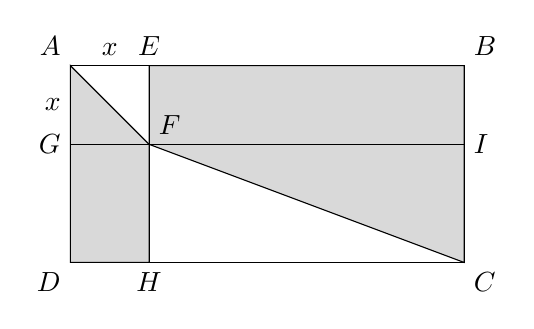
\begin{tikzpicture}
\coordinate (A) at (0,0);
\coordinate (B) at (5,0);
\coordinate (C) at (5,-2.5);
\coordinate (D) at (0,-2.5);

\coordinate (E) at (1,0);
\coordinate (G) at (0,-1);
\coordinate (F) at (1,-1);

\coordinate (I) at (5,-1);
\coordinate (H) at (1,-2.5);

\fill[color=gray!30] (A) -- (F) -- (H) -- (D) -- cycle;
\draw (A) -- (F) -- (H) -- (D) -- cycle;
\fill[color=gray!30] (E) -- (F) -- (C) -- (B) -- cycle;
\draw (E) -- (F) -- (C) -- (B) -- cycle;

\draw (A) -- (B) -- (C) -- (D) -- cycle;
\draw (A) -- (E) -- (F) -- (G) -- cycle;
\draw (F) -- (I) -- (C) -- (H) -- cycle;

\draw (A) node[above left] {$A$};
\draw (B) node[above right] {$B$};
\draw (C) node[below right] {$C$};
\draw (D) node[below left] {$D$};
\draw (E) node[above] {$E$};
\draw (G) node[left] {$G$};
\draw (F) node[above right] {$F$};
\draw (I) node[right] {$I$};
\draw (H) node[below] {$H$};

\draw (A) -- (G) node[midway,left] {$x$};
\draw (A) -- (E) node[midway,above] {$x$};
\end{tikzpicture}
\end{center}
\begin{parts}
\part[1] Justifier que $x$ est dans l'intervalle $[0;6]$.
\begin{solution}
$G$ est un point du segment $[AD]$, la longueur $x$ du segment $[AG]$ ne peut donc pas dépasser la longueur $AD = 6$.

De plus, $x$ est une longueur, et est donc positive.

On en déduit donc que $x \in [0;6]$.
\end{solution}
\part[2] Démontrer alors que pour tout $x \in [0;6]$,
\begin{equation*}
M(x) = x^2 - 8x + 30  
\end{equation*}
\begin{solution}
$M(x)$ est donné par l'aire du triangle rectangle $AEF$ et du triangle $HFC$.

Alors,
\begin{equation*}
\begin{aligned}
M(x) &= \dfrac{AE \times EF}{2} + \dfrac{HF \times HC}{2}\\
&= \dfrac{x \times x}{2} + \dfrac{(10 - x) \times (6 - x)}{2}\\
&= \dfrac{x^2}{2} + \dfrac{60 - 16x + x^2}{2}\\
&= \dfrac{x^2}{2} + \dfrac{60}{2} - \dfrac{16x}{2} + \dfrac{x^2}{2}\\
&= x^2 - 8x + 30 
\end{aligned}
\end{equation*}
\end{solution}

\part[1] Tracer le tableau de variations de l'aire laissée blanche. 

En déduire la valeur de $x$ pour laquelle cette aire est minimale.
\begin{solution}
On écrit l'expression de l'aire $M(x) = x^2 - 8x + 30$ sous forme canonique.

\begin{equation*}
\begin{aligned}
M(x) &= x^2 - 8x + 30\\
&= (x - 4)^2 - 16 + 30\\
&= (x - 4)^2 + 14
\end{aligned}
\end{equation*}
On en déduit que $\alpha = 4$ et $\beta = 14$. De plus, comme $a = 1 > 0$, on en déduit que
\begin{center}
\begin{tikzpicture}
\tkzTabInit{$x$/1, Variations de $f$/2}{$-\infty$, $4$, $+\infty$};
\tkzTabVar{+/, -/$14$, +/}
\end{tikzpicture}
\end{center}
\end{solution}
\part[2] Montrer que quelque soit la valeur de $x$, l'aire blanche est toujours supérieure à l'aire du rectangle $GFDH$. (Indication : Si on pose $N(x)$ l'aire de $GFDH$, on étudiera le signe $M(x) - N(x)$)
\begin{solution}
On pose $N(x)$ l'expression de l'aire de $GDFH$. Alors, pour tout $x \in [0;6]$,
\begin{equation*}
N(x) = GD \times HD = (6 - x) \times x = -x^2 + 6x
\end{equation*}
On souhaite donc montrer que pour tout $x \in [0,6]$, $M(x) > N(x)$. Cela est équivalent à montrer que $M(x) - N(x) > 0$.

On s'intéresse à $M(x) - N(x)$,
\begin{equation*}
\begin{aligned}
M(x) - N(x) &= x^2 - 8x + 30 - (- x^2 + 6x)\\
&= x^2 - 8x + 30 + x^2 - 6x\\
&= 2x^2 -14x + 30\\
&= 2(x^2 - 7x) + 30\\
&= 2((x - 3,5)^2 - 12,25) + 30\\
&= 2(x-3,5)^2 + 17,75
\end{aligned}
\end{equation*}
En mettant $M(x) - N(x)$ sous forme canonique, on constate que $\beta = 17,75$. De plus, ici, $a = 2 > 0$, ce qui signifie que cette fonction admet un minimum supérieur à $0$. On en déduit que $M(x) - N(x)$ est positif pour tout $x \in [0;6]$. On a donc démontré le résultat souhaité.
\end{solution}  
\end{parts}
\end{questions}
\end{document}